% Options for packages loaded elsewhere
\PassOptionsToPackage{unicode}{hyperref}
\PassOptionsToPackage{hyphens}{url}
\documentclass[
]{article}
\usepackage{xcolor}
\usepackage[margin=1in]{geometry}
\usepackage{amsmath,amssymb}
\setcounter{secnumdepth}{-\maxdimen} % remove section numbering
\usepackage{iftex}
\ifPDFTeX
  \usepackage[T1]{fontenc}
  \usepackage[utf8]{inputenc}
  \usepackage{textcomp} % provide euro and other symbols
\else % if luatex or xetex
  \usepackage{unicode-math} % this also loads fontspec
  \defaultfontfeatures{Scale=MatchLowercase}
  \defaultfontfeatures[\rmfamily]{Ligatures=TeX,Scale=1}
\fi
\usepackage{lmodern}
\ifPDFTeX\else
  % xetex/luatex font selection
\fi
% Use upquote if available, for straight quotes in verbatim environments
\IfFileExists{upquote.sty}{\usepackage{upquote}}{}
\IfFileExists{microtype.sty}{% use microtype if available
  \usepackage[]{microtype}
  \UseMicrotypeSet[protrusion]{basicmath} % disable protrusion for tt fonts
}{}
\makeatletter
\@ifundefined{KOMAClassName}{% if non-KOMA class
  \IfFileExists{parskip.sty}{%
    \usepackage{parskip}
  }{% else
    \setlength{\parindent}{0pt}
    \setlength{\parskip}{6pt plus 2pt minus 1pt}}
}{% if KOMA class
  \KOMAoptions{parskip=half}}
\makeatother
\usepackage{color}
\usepackage{fancyvrb}
\newcommand{\VerbBar}{|}
\newcommand{\VERB}{\Verb[commandchars=\\\{\}]}
\DefineVerbatimEnvironment{Highlighting}{Verbatim}{commandchars=\\\{\}}
% Add ',fontsize=\small' for more characters per line
\usepackage{framed}
\definecolor{shadecolor}{RGB}{248,248,248}
\newenvironment{Shaded}{\begin{snugshade}}{\end{snugshade}}
\newcommand{\AlertTok}[1]{\textcolor[rgb]{0.94,0.16,0.16}{#1}}
\newcommand{\AnnotationTok}[1]{\textcolor[rgb]{0.56,0.35,0.01}{\textbf{\textit{#1}}}}
\newcommand{\AttributeTok}[1]{\textcolor[rgb]{0.13,0.29,0.53}{#1}}
\newcommand{\BaseNTok}[1]{\textcolor[rgb]{0.00,0.00,0.81}{#1}}
\newcommand{\BuiltInTok}[1]{#1}
\newcommand{\CharTok}[1]{\textcolor[rgb]{0.31,0.60,0.02}{#1}}
\newcommand{\CommentTok}[1]{\textcolor[rgb]{0.56,0.35,0.01}{\textit{#1}}}
\newcommand{\CommentVarTok}[1]{\textcolor[rgb]{0.56,0.35,0.01}{\textbf{\textit{#1}}}}
\newcommand{\ConstantTok}[1]{\textcolor[rgb]{0.56,0.35,0.01}{#1}}
\newcommand{\ControlFlowTok}[1]{\textcolor[rgb]{0.13,0.29,0.53}{\textbf{#1}}}
\newcommand{\DataTypeTok}[1]{\textcolor[rgb]{0.13,0.29,0.53}{#1}}
\newcommand{\DecValTok}[1]{\textcolor[rgb]{0.00,0.00,0.81}{#1}}
\newcommand{\DocumentationTok}[1]{\textcolor[rgb]{0.56,0.35,0.01}{\textbf{\textit{#1}}}}
\newcommand{\ErrorTok}[1]{\textcolor[rgb]{0.64,0.00,0.00}{\textbf{#1}}}
\newcommand{\ExtensionTok}[1]{#1}
\newcommand{\FloatTok}[1]{\textcolor[rgb]{0.00,0.00,0.81}{#1}}
\newcommand{\FunctionTok}[1]{\textcolor[rgb]{0.13,0.29,0.53}{\textbf{#1}}}
\newcommand{\ImportTok}[1]{#1}
\newcommand{\InformationTok}[1]{\textcolor[rgb]{0.56,0.35,0.01}{\textbf{\textit{#1}}}}
\newcommand{\KeywordTok}[1]{\textcolor[rgb]{0.13,0.29,0.53}{\textbf{#1}}}
\newcommand{\NormalTok}[1]{#1}
\newcommand{\OperatorTok}[1]{\textcolor[rgb]{0.81,0.36,0.00}{\textbf{#1}}}
\newcommand{\OtherTok}[1]{\textcolor[rgb]{0.56,0.35,0.01}{#1}}
\newcommand{\PreprocessorTok}[1]{\textcolor[rgb]{0.56,0.35,0.01}{\textit{#1}}}
\newcommand{\RegionMarkerTok}[1]{#1}
\newcommand{\SpecialCharTok}[1]{\textcolor[rgb]{0.81,0.36,0.00}{\textbf{#1}}}
\newcommand{\SpecialStringTok}[1]{\textcolor[rgb]{0.31,0.60,0.02}{#1}}
\newcommand{\StringTok}[1]{\textcolor[rgb]{0.31,0.60,0.02}{#1}}
\newcommand{\VariableTok}[1]{\textcolor[rgb]{0.00,0.00,0.00}{#1}}
\newcommand{\VerbatimStringTok}[1]{\textcolor[rgb]{0.31,0.60,0.02}{#1}}
\newcommand{\WarningTok}[1]{\textcolor[rgb]{0.56,0.35,0.01}{\textbf{\textit{#1}}}}
\usepackage{graphicx}
\makeatletter
\newsavebox\pandoc@box
\newcommand*\pandocbounded[1]{% scales image to fit in text height/width
  \sbox\pandoc@box{#1}%
  \Gscale@div\@tempa{\textheight}{\dimexpr\ht\pandoc@box+\dp\pandoc@box\relax}%
  \Gscale@div\@tempb{\linewidth}{\wd\pandoc@box}%
  \ifdim\@tempb\p@<\@tempa\p@\let\@tempa\@tempb\fi% select the smaller of both
  \ifdim\@tempa\p@<\p@\scalebox{\@tempa}{\usebox\pandoc@box}%
  \else\usebox{\pandoc@box}%
  \fi%
}
% Set default figure placement to htbp
\def\fps@figure{htbp}
\makeatother
\setlength{\emergencystretch}{3em} % prevent overfull lines
\providecommand{\tightlist}{%
  \setlength{\itemsep}{0pt}\setlength{\parskip}{0pt}}
\usepackage{booktabs}
\usepackage{longtable}
\usepackage{array}
\usepackage{multirow}
\usepackage{wrapfig}
\usepackage{float}
\usepackage{colortbl}
\usepackage{pdflscape}
\usepackage{tabu}
\usepackage{threeparttable}
\usepackage{threeparttablex}
\usepackage[normalem]{ulem}
\usepackage{makecell}
\usepackage{xcolor}
\usepackage{bookmark}
\IfFileExists{xurl.sty}{\usepackage{xurl}}{} % add URL line breaks if available
\urlstyle{same}
\hypersetup{
  pdftitle={Data Science I Homework 2},
  hidelinks,
  pdfcreator={LaTeX via pandoc}}

\title{Data Science I Homework 2}
\author{}
\date{\vspace{-2.5em}}

\begin{document}
\maketitle

\section{Question 1}\label{question-1}

\begin{Shaded}
\begin{Highlighting}[]
\CommentTok{\#load the necessary packages\#}

\FunctionTok{library}\NormalTok{(tidyverse)}
\end{Highlighting}
\end{Shaded}

\begin{verbatim}
## -- Attaching core tidyverse packages ------------------------ tidyverse 2.0.0 --
## v dplyr     1.1.4     v readr     2.1.5
## v forcats   1.0.0     v stringr   1.5.1
## v ggplot2   3.5.2     v tibble    3.3.0
## v lubridate 1.9.4     v tidyr     1.3.1
## v purrr     1.1.0     
## -- Conflicts ------------------------------------------ tidyverse_conflicts() --
## x dplyr::filter() masks stats::filter()
## x dplyr::lag()    masks stats::lag()
## i Use the conflicted package (<http://conflicted.r-lib.org/>) to force all conflicts to become errors
\end{verbatim}

\begin{Shaded}
\begin{Highlighting}[]
\FunctionTok{library}\NormalTok{(ggridges)}
\FunctionTok{library}\NormalTok{(patchwork)}
\FunctionTok{library}\NormalTok{(kableExtra)}
\end{Highlighting}
\end{Shaded}

\begin{verbatim}
## 
## Attaching package: 'kableExtra'
## 
## The following object is masked from 'package:dplyr':
## 
##     group_rows
\end{verbatim}

\begin{Shaded}
\begin{Highlighting}[]
\CommentTok{\#load the p8105 dataset and instacart\#}

\FunctionTok{library}\NormalTok{(p8105.datasets)}
\FunctionTok{data}\NormalTok{(}\StringTok{"instacart"}\NormalTok{)}

\CommentTok{\#count the amount of times an aisle appears\#}

\NormalTok{instacart }\SpecialCharTok{\%\textgreater{}\%} \FunctionTok{count}\NormalTok{(aisle, }\AttributeTok{sort =} \ConstantTok{TRUE}\NormalTok{)}
\end{Highlighting}
\end{Shaded}

\begin{verbatim}
## # A tibble: 134 x 2
##    aisle                              n
##    <chr>                          <int>
##  1 fresh vegetables              150609
##  2 fresh fruits                  150473
##  3 packaged vegetables fruits     78493
##  4 yogurt                         55240
##  5 packaged cheese                41699
##  6 water seltzer sparkling water  36617
##  7 milk                           32644
##  8 chips pretzels                 31269
##  9 soy lactosefree                26240
## 10 bread                          23635
## # i 124 more rows
\end{verbatim}

There are about 134aisles in total. The aisle with the most amount of
items ordered would be fresh vegetables.

\begin{Shaded}
\begin{Highlighting}[]
\CommentTok{\#Produce a plot for the amount of times an item was ordered from an aisle\#}

\NormalTok{instacart }\SpecialCharTok{|\textgreater{}} \FunctionTok{count}\NormalTok{(aisle, }\AttributeTok{sort =} \ConstantTok{TRUE}\NormalTok{) }\SpecialCharTok{|\textgreater{}} \FunctionTok{filter}\NormalTok{(n }\SpecialCharTok{\textgreater{}} \DecValTok{10000}\NormalTok{) }\SpecialCharTok{|\textgreater{}}
  \FunctionTok{mutate}\NormalTok{(}\AttributeTok{aisle =} \FunctionTok{reorder}\NormalTok{(aisle, n)) }\SpecialCharTok{|\textgreater{}} \FunctionTok{ggplot}\NormalTok{(}\FunctionTok{aes}\NormalTok{(}\AttributeTok{x =}\NormalTok{ n, }\AttributeTok{y =}\NormalTok{ aisle)) }\SpecialCharTok{+}
  \FunctionTok{geom\_col}\NormalTok{() }\SpecialCharTok{+}  \FunctionTok{labs}\NormalTok{(}\AttributeTok{title =} \StringTok{"Total Number of Items Ordered for Each Aisle"}\NormalTok{, }\AttributeTok{x =} \StringTok{"Total Number of Items Ordered"}\NormalTok{, }\AttributeTok{y =} \StringTok{"Aisle"}\NormalTok{)}
\end{Highlighting}
\end{Shaded}

\pandocbounded{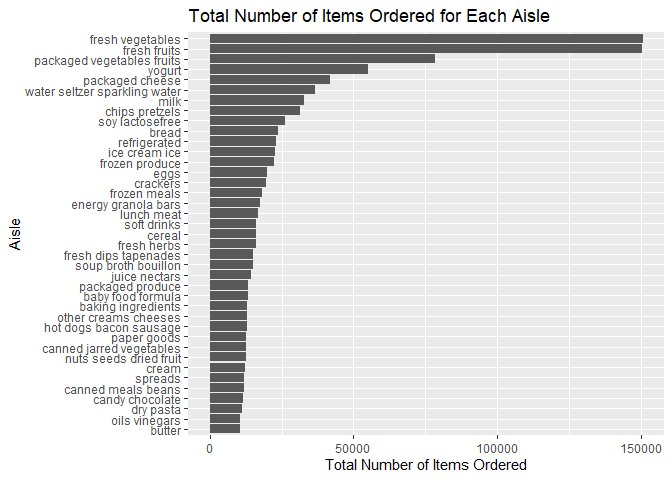
\includegraphics[keepaspectratio]{p8105_hw3_ry2539_files/figure-latex/aisle_items_ordered-1.pdf}}

The most popular items that are ordered seems to be from aisles that are
relevant to necessary groceries. This include not only vegetables and
fruits, but also dairy products like milk and cheese. Frozen produce and
eggs are also popularly ordered. The less popular items ordered have to
do with sugars and additional sources of protein and starch.

\begin{Shaded}
\begin{Highlighting}[]
\CommentTok{\#Make a table that shows the amount of times the 3 most popular items were ordered from each aisle\#}

\NormalTok{instacart }\SpecialCharTok{|\textgreater{}} \FunctionTok{filter}\NormalTok{(aisle }\SpecialCharTok{==} \StringTok{"packaged vegetables fruits"} \SpecialCharTok{|}\NormalTok{ aisle }\SpecialCharTok{==} \StringTok{"dog food care"} \SpecialCharTok{|}
\NormalTok{                      aisle }\SpecialCharTok{==} \StringTok{"baking ingredients"}\NormalTok{) }\SpecialCharTok{|\textgreater{}} 
                      \FunctionTok{count}\NormalTok{(aisle, product\_name, }\AttributeTok{sort =} \ConstantTok{TRUE}\NormalTok{) }\SpecialCharTok{|\textgreater{}} \FunctionTok{group\_by}\NormalTok{(aisle) }\SpecialCharTok{|\textgreater{}}
                      \FunctionTok{slice\_max}\NormalTok{(}\AttributeTok{order\_by =}\NormalTok{ n, }\AttributeTok{n =} \DecValTok{3}\NormalTok{) }\SpecialCharTok{|\textgreater{}}
                      \FunctionTok{arrange}\NormalTok{(aisle, n) }\SpecialCharTok{|\textgreater{}}
                      \FunctionTok{mutate}\NormalTok{(}\StringTok{\textasciigrave{}}\AttributeTok{Number of Times Ordered}\StringTok{\textasciigrave{}} \OtherTok{=}\NormalTok{ n) }\SpecialCharTok{|\textgreater{}}
                      \FunctionTok{select}\NormalTok{(}\SpecialCharTok{{-}}\NormalTok{n)}
\end{Highlighting}
\end{Shaded}

\begin{verbatim}
## # A tibble: 9 x 3
## # Groups:   aisle [3]
##   aisle                      product_name                 Number of Times Orde~1
##   <chr>                      <chr>                                         <int>
## 1 baking ingredients         Cane Sugar                                      336
## 2 baking ingredients         Pure Baking Soda                                387
## 3 baking ingredients         Light Brown Sugar                               499
## 4 dog food care              Small Dog Biscuits                               26
## 5 dog food care              Organix Chicken & Brown Ric~                     28
## 6 dog food care              Snack Sticks Chicken & Rice~                     30
## 7 packaged vegetables fruits Organic Blueberries                            4966
## 8 packaged vegetables fruits Organic Raspberries                            5546
## 9 packaged vegetables fruits Organic Baby Spinach                           9784
## # i abbreviated name: 1: `Number of Times Ordered`
\end{verbatim}

Among the three aisles, dog food care has the least amount of items
ordered from it. This can be explained by how only a portion of
customers own pets--and only a portion own dogs--and thus a smaller
proportion of customers would need dog food. With that said, the most
popular item in this aisle is Snack Sticks Chicken \& Rice Recipe Dog
Treats.

Meanwhile, packaged vegetable fruits is the most popular aisle due to
how such items do not need further preparation to eat, as opposed to
baking ingredients that require work on the customers. The most popular
item from this aisle is organic baby spinach. This could be because
organic baby spinach can be eaten raw and cooked, giving it more
variety. It is also interesting to note that customers seem to prefer
raspberries to blueberries.

Finally, among baking ingredients, customer seem to prefer light brown
sugar compared to cane sugar. This could be due to how light brown sugar
is refined and could give a richer flavor compared to cane sugar.

\begin{Shaded}
\begin{Highlighting}[]
\CommentTok{\#produce a reader friendly table for the specific time on the specific day our two products were ordered on average\#}

\NormalTok{instacart }\SpecialCharTok{|\textgreater{}} \FunctionTok{filter}\NormalTok{(product\_name }\SpecialCharTok{==} \StringTok{"Pink Lady Apples"} \SpecialCharTok{|}\NormalTok{ product\_name }\SpecialCharTok{==} \StringTok{"Coffee Ice Cream"}\NormalTok{) }\SpecialCharTok{|\textgreater{}} \FunctionTok{mutate}\NormalTok{(}\AttributeTok{order\_dow =} \FunctionTok{case\_when}\NormalTok{(}
\NormalTok{            order\_dow }\SpecialCharTok{==} \DecValTok{0} \SpecialCharTok{\textasciitilde{}} \StringTok{"Sunday"}\NormalTok{,}
\NormalTok{            order\_dow }\SpecialCharTok{==} \DecValTok{1} \SpecialCharTok{\textasciitilde{}} \StringTok{"Monday"}\NormalTok{,}
\NormalTok{            order\_dow }\SpecialCharTok{==} \DecValTok{2} \SpecialCharTok{\textasciitilde{}} \StringTok{"Tuesday"}\NormalTok{,}
\NormalTok{            order\_dow }\SpecialCharTok{==} \DecValTok{3} \SpecialCharTok{\textasciitilde{}} \StringTok{"Wednesday"}\NormalTok{,}
\NormalTok{            order\_dow }\SpecialCharTok{==} \DecValTok{4} \SpecialCharTok{\textasciitilde{}} \StringTok{"Thursday"}\NormalTok{,}
\NormalTok{            order\_dow }\SpecialCharTok{==} \DecValTok{5} \SpecialCharTok{\textasciitilde{}} \StringTok{"Friday"}\NormalTok{,}
\NormalTok{            order\_dow }\SpecialCharTok{==} \DecValTok{6} \SpecialCharTok{\textasciitilde{}} \StringTok{"Saturday"}\NormalTok{,}
\NormalTok{          )) }\SpecialCharTok{|\textgreater{}} \FunctionTok{group\_by}\NormalTok{(product\_name, order\_dow) }\SpecialCharTok{|\textgreater{}}
          \FunctionTok{summarize}\NormalTok{(}\AttributeTok{mean\_hour =} \FunctionTok{mean}\NormalTok{(order\_hour\_of\_day)) }\SpecialCharTok{|\textgreater{}}
          \FunctionTok{pivot\_wider}\NormalTok{(}
            \AttributeTok{names\_from =}\NormalTok{ order\_dow,}
            \AttributeTok{values\_from =}\NormalTok{ mean\_hour}
\NormalTok{          )}
\end{Highlighting}
\end{Shaded}

\begin{verbatim}
## `summarise()` has grouped output by 'product_name'. You can override using the
## `.groups` argument.
\end{verbatim}

\begin{verbatim}
## # A tibble: 2 x 8
## # Groups:   product_name [2]
##   product_name     Friday Monday Saturday Sunday Thursday Tuesday Wednesday
##   <chr>             <dbl>  <dbl>    <dbl>  <dbl>    <dbl>   <dbl>     <dbl>
## 1 Coffee Ice Cream   12.3   14.3     13.8   13.8     15.2    15.4      15.3
## 2 Pink Lady Apples   12.8   11.4     11.9   13.4     11.6    11.7      14.2
\end{verbatim}

Both products seem to be ordered around the afternoon on Friday, Sunday,
and Wednesday. However, aside from Friday when Pink Lady Apples is
ordered after Coffee Ice Cream, Pink Lady Apples is ordered before
Coffee Ice Cream on Sunday and Wednesday. On every other day, while
Coffee Ice Cream is still ordered around the afternoon, Pink Lady Apples
is ordered around late morning before the noon. This could be because
Pink Lady Apples is a fruit and would be in popular demand. Therefore,
customers would likely want to order such an item as early as possible.
Meanwhile, Coffee Ice Cream would be suited to when the day is hot,
which is likely to happen in the afternoon.

\section{Question 2}\label{question-2}

\begin{Shaded}
\begin{Highlighting}[]
\CommentTok{\#Read the zillow rental price data file\#}

\NormalTok{zillow\_price\_df }\OtherTok{=} \FunctionTok{read\_csv}\NormalTok{(}\StringTok{"./zillow\_data/zillow\_data/Zip\_zori\_uc\_sfrcondomfr\_sm\_month\_NYC.csv"}\NormalTok{)}
\end{Highlighting}
\end{Shaded}

\begin{verbatim}
## Rows: 149 Columns: 125
## -- Column specification --------------------------------------------------------
## Delimiter: ","
## chr   (6): RegionType, StateName, State, City, Metro, CountyName
## dbl (119): RegionID, SizeRank, RegionName, 2015-01-31, 2015-02-28, 2015-03-3...
## 
## i Use `spec()` to retrieve the full column specification for this data.
## i Specify the column types or set `show_col_types = FALSE` to quiet this message.
\end{verbatim}

\begin{Shaded}
\begin{Highlighting}[]
\CommentTok{\#Have a new data variable as ZipCode from the regionname variable\#}

\NormalTok{zillow\_price\_zip\_variation\_df }\OtherTok{=} \FunctionTok{mutate}\NormalTok{(zillow\_price\_df, }\AttributeTok{ZipCode =}\NormalTok{ RegionName)}

\CommentTok{\#Clean the data and eliminate StateName, RegionName, RegionType, which are unnecessary data variables\#}

\NormalTok{zillow\_clean\_price\_df }\OtherTok{=} \FunctionTok{select}\NormalTok{(zillow\_price\_zip\_variation\_df, }\SpecialCharTok{{-}}\StringTok{\textasciigrave{}}\AttributeTok{StateName}\StringTok{\textasciigrave{}}\NormalTok{, }\SpecialCharTok{{-}}\NormalTok{RegionName, }\SpecialCharTok{{-}}\NormalTok{RegionType)}
\end{Highlighting}
\end{Shaded}

\begin{Shaded}
\begin{Highlighting}[]
\CommentTok{\#Read the zillow properties data file\#}

\NormalTok{zillow\_df }\OtherTok{=} \FunctionTok{read\_csv}\NormalTok{(}\StringTok{"./zillow\_data/zillow\_data/Zip Codes.csv"}\NormalTok{)}
\end{Highlighting}
\end{Shaded}

\begin{verbatim}
## Rows: 322 Columns: 7
## -- Column specification --------------------------------------------------------
## Delimiter: ","
## chr (4): County, County Code, File Date, Neighborhood
## dbl (3): State FIPS, County FIPS, ZipCode
## 
## i Use `spec()` to retrieve the full column specification for this data.
## i Specify the column types or set `show_col_types = FALSE` to quiet this message.
\end{verbatim}

\begin{Shaded}
\begin{Highlighting}[]
\CommentTok{\#Mutate the CountyName variable from "Bronx" to "Bronx County"\#}

\NormalTok{zillow\_county\_variation\_df }\OtherTok{=} \FunctionTok{mutate}\NormalTok{(zillow\_df, }\AttributeTok{CountyName =} \FunctionTok{paste}\NormalTok{(County, }\StringTok{"County"}\NormalTok{))}

\CommentTok{\#Eliminate varibles such as State FIPS, County FIPS, and County\#}

\NormalTok{zillow\_clean\_df }\OtherTok{=} \FunctionTok{select}\NormalTok{(zillow\_county\_variation\_df, }\SpecialCharTok{{-}}\StringTok{\textasciigrave{}}\AttributeTok{State FIPS}\StringTok{\textasciigrave{}}\NormalTok{, }\SpecialCharTok{{-}}\StringTok{\textasciigrave{}}\AttributeTok{County FIPS}\StringTok{\textasciigrave{}}\NormalTok{, }\SpecialCharTok{{-}}\NormalTok{County)}
\end{Highlighting}
\end{Shaded}

\begin{Shaded}
\begin{Highlighting}[]
\CommentTok{\#Merge the two datasets into a single tidy dataset\#}

\NormalTok{first\_single\_zillow\_df }\OtherTok{=} \FunctionTok{left\_join}\NormalTok{(zillow\_clean\_df, zillow\_clean\_price\_df)}
\end{Highlighting}
\end{Shaded}

\begin{verbatim}
## Joining with `by = join_by(ZipCode, CountyName)`
\end{verbatim}

\begin{Shaded}
\begin{Highlighting}[]
\NormalTok{first\_clean\_single\_zillow\_df }\OtherTok{=} \FunctionTok{arrange}\NormalTok{(first\_single\_zillow\_df, RegionID)}

\CommentTok{\#Use pivot longer to see rental price for each year and month for each zip code\#}

\NormalTok{pivot\_longer\_single\_zillow\_df }\OtherTok{=} \FunctionTok{pivot\_longer}\NormalTok{(}
\NormalTok{  first\_clean\_single\_zillow\_df, }\AttributeTok{cols =} \FunctionTok{starts\_with}\NormalTok{(}\StringTok{"20"}\NormalTok{),}
  \AttributeTok{names\_to =} \StringTok{"Date"}\NormalTok{,}
  \AttributeTok{values\_to =} \StringTok{"Rental Price"}
\NormalTok{)}

\CommentTok{\#make a table that shows how many times a zip code is observed\#}

\NormalTok{not\_na\_pivot\_longer\_zillow\_df }\OtherTok{=}\NormalTok{ pivot\_longer\_single\_zillow\_df }\SpecialCharTok{\%\textgreater{}\%} \FunctionTok{drop\_na}\NormalTok{(}\StringTok{\textasciigrave{}}\AttributeTok{Rental Price}\StringTok{\textasciigrave{}}\NormalTok{)}
\NormalTok{is\_na\_pivot\_longer\_zillow\_df }\OtherTok{=}\NormalTok{ pivot\_longer\_single\_zillow\_df }\SpecialCharTok{\%\textgreater{}\%} \FunctionTok{filter}\NormalTok{(}\FunctionTok{is.na}\NormalTok{(}\StringTok{\textasciigrave{}}\AttributeTok{Rental Price}\StringTok{\textasciigrave{}}\NormalTok{))}

\NormalTok{not\_na\_pivot\_longer\_single\_zillow\_df }\OtherTok{=} 
\NormalTok{  not\_na\_pivot\_longer\_zillow\_df }\SpecialCharTok{|\textgreater{}} \FunctionTok{count}\NormalTok{(ZipCode, }\AttributeTok{sort =} \ConstantTok{TRUE}\NormalTok{)}

\NormalTok{is\_na\_pivot\_longer\_single\_zillow\_df }\OtherTok{=}
\NormalTok{  is\_na\_pivot\_longer\_zillow\_df }\SpecialCharTok{|\textgreater{}} \FunctionTok{count}\NormalTok{(ZipCode, }\AttributeTok{sort =} \ConstantTok{TRUE}\NormalTok{)}

\NormalTok{is\_na\_pivot\_longer\_single\_zillow\_df }\OtherTok{=}\NormalTok{ is\_na\_pivot\_longer\_single\_zillow\_df }\SpecialCharTok{\%\textgreater{}\%} \FunctionTok{mutate}\NormalTok{(}\AttributeTok{n =} \DecValTok{0}\NormalTok{)}

\NormalTok{combined\_zip\_code\_rental\_count\_df }\OtherTok{=} \FunctionTok{bind\_rows}\NormalTok{(is\_na\_pivot\_longer\_single\_zillow\_df, not\_na\_pivot\_longer\_single\_zillow\_df)}

\NormalTok{counts\_of\_zip\_codes }\OtherTok{=}\NormalTok{ combined\_zip\_code\_rental\_count\_df }\SpecialCharTok{\%\textgreater{}\%} \FunctionTok{group\_by}\NormalTok{(ZipCode) }\SpecialCharTok{\%\textgreater{}\%}
  \FunctionTok{summarise}\NormalTok{(}\AttributeTok{n =} \FunctionTok{sum}\NormalTok{(n))}

\CommentTok{\#get the highest counts and lowest counts of zip codes\#}

\NormalTok{highest\_counts\_of\_zip\_codes }\OtherTok{=}\NormalTok{ counts\_of\_zip\_codes }\SpecialCharTok{\%\textgreater{}\%} \FunctionTok{filter}\NormalTok{(n }\SpecialCharTok{==} \DecValTok{116}\NormalTok{)}
\NormalTok{lowest\_counts\_of\_zip\_codes }\OtherTok{=}\NormalTok{ counts\_of\_zip\_codes }\SpecialCharTok{\%\textgreater{}\%} \FunctionTok{filter}\NormalTok{(n }\SpecialCharTok{\textless{}} \DecValTok{10}\NormalTok{) }\SpecialCharTok{\%\textgreater{}\%} \FunctionTok{arrange}\NormalTok{(}\FunctionTok{desc}\NormalTok{(n))}
\end{Highlighting}
\end{Shaded}

The number of ZIP codes that were observed for all 116 months is 48.
Meanwhile, the number of ZIP codes that were observed for fewer than 10
months is 197. A lot of the zip codes that were observed rarely are
located in areas of NYC that host a lot of business. Therefore, these
properties would likely not have rental prices, as these buildings would
already be occupied for various companies. Meanwhile, other zip codes
that are observed each month take place in locations such as upper
Manhattan and Brooklyn, where residential buildings would be more
concentrated in.

\begin{Shaded}
\begin{Highlighting}[]
\NormalTok{Year\_pivot\_longer\_df }\OtherTok{=} \FunctionTok{separate}\NormalTok{(pivot\_longer\_single\_zillow\_df, }
\NormalTok{                                Date, }\AttributeTok{into =} \FunctionTok{c}\NormalTok{(}\StringTok{"Year"}\NormalTok{, }\StringTok{"Month"}\NormalTok{, }\StringTok{"Day"}\NormalTok{), }\AttributeTok{sep =} \StringTok{"{-}"}\NormalTok{)}

\NormalTok{Year\_1\_pivot\_longer\_df }\OtherTok{=}\NormalTok{ Year\_pivot\_longer\_df }\SpecialCharTok{|\textgreater{}} \FunctionTok{mutate}\NormalTok{(}\AttributeTok{Year =} \FunctionTok{strtoi}\NormalTok{(Year))}

\CommentTok{\#Create table that shows mean rental price for all boroughs\#}

\NormalTok{Year\_Borough\_df }\OtherTok{=}\NormalTok{ Year\_1\_pivot\_longer\_df }\SpecialCharTok{|\textgreater{}} \FunctionTok{drop\_na}\NormalTok{(}\StringTok{\textasciigrave{}}\AttributeTok{Rental Price}\StringTok{\textasciigrave{}}\NormalTok{) }\SpecialCharTok{|\textgreater{}} \FunctionTok{group\_by}\NormalTok{(Year, CountyName) }\SpecialCharTok{|\textgreater{}}
  \FunctionTok{summarize}\NormalTok{(}\AttributeTok{mean\_rental\_price =} \FunctionTok{mean}\NormalTok{(}\StringTok{\textasciigrave{}}\AttributeTok{Rental Price}\StringTok{\textasciigrave{}}\NormalTok{, }\AttributeTok{na.rm =} \ConstantTok{TRUE}\NormalTok{)) }\SpecialCharTok{|\textgreater{}} \FunctionTok{arrange}\NormalTok{(CountyName)}
\end{Highlighting}
\end{Shaded}

\begin{verbatim}
## `summarise()` has grouped output by 'Year'. You can override using the
## `.groups` argument.
\end{verbatim}

\begin{Shaded}
\begin{Highlighting}[]
\NormalTok{Year\_Borough\_df}
\end{Highlighting}
\end{Shaded}

\begin{verbatim}
## # A tibble: 45 x 3
## # Groups:   Year [10]
##     Year CountyName   mean_rental_price
##    <int> <chr>                    <dbl>
##  1  2015 Bronx County             1760.
##  2  2016 Bronx County             1520.
##  3  2017 Bronx County             1544.
##  4  2018 Bronx County             1639.
##  5  2019 Bronx County             1706.
##  6  2020 Bronx County             1811.
##  7  2021 Bronx County             1858.
##  8  2022 Bronx County             2054.
##  9  2023 Bronx County             2285.
## 10  2024 Bronx County             2497.
## # i 35 more rows
\end{verbatim}

\begin{Shaded}
\begin{Highlighting}[]
\FunctionTok{ggplot}\NormalTok{(Year\_Borough\_df, }\FunctionTok{aes}\NormalTok{(}\AttributeTok{x =}\NormalTok{ Year, }\AttributeTok{y =}\NormalTok{ mean\_rental\_price)) }\SpecialCharTok{+} \FunctionTok{geom\_point}\NormalTok{(}\FunctionTok{aes}\NormalTok{(}\AttributeTok{color =}\NormalTok{ CountyName), }\AttributeTok{alpha =} \FloatTok{0.5}\NormalTok{) }\SpecialCharTok{+}
  \FunctionTok{geom\_smooth}\NormalTok{(}\AttributeTok{se =} \ConstantTok{FALSE}\NormalTok{) }\SpecialCharTok{+} \FunctionTok{facet\_grid}\NormalTok{(.}\SpecialCharTok{\textasciitilde{}}\NormalTok{CountyName) }\SpecialCharTok{+} \FunctionTok{labs}\NormalTok{(}\AttributeTok{title =} \StringTok{"Mean Rental Price Across the Years for All Boroughs"}\NormalTok{, }\AttributeTok{x =} \StringTok{"Year"}\NormalTok{, }\AttributeTok{y =} \StringTok{"Mean Rental Price"}\NormalTok{, }\AttributeTok{color =} \StringTok{"Boroughs"}\NormalTok{)}
\end{Highlighting}
\end{Shaded}

\begin{verbatim}
## `geom_smooth()` using method = 'loess' and formula = 'y ~ x'
\end{verbatim}

\begin{verbatim}
## Warning in simpleLoess(y, x, w, span, degree = degree, parametric = parametric,
## : span too small.  fewer data values than degrees of freedom.
\end{verbatim}

\begin{verbatim}
## Warning in simpleLoess(y, x, w, span, degree = degree, parametric = parametric,
## : pseudoinverse used at 2020
\end{verbatim}

\begin{verbatim}
## Warning in simpleLoess(y, x, w, span, degree = degree, parametric = parametric,
## : neighborhood radius 2.02
\end{verbatim}

\begin{verbatim}
## Warning in simpleLoess(y, x, w, span, degree = degree, parametric = parametric,
## : reciprocal condition number 0
\end{verbatim}

\begin{verbatim}
## Warning in simpleLoess(y, x, w, span, degree = degree, parametric = parametric,
## : There are other near singularities as well. 4.0804
\end{verbatim}

\pandocbounded{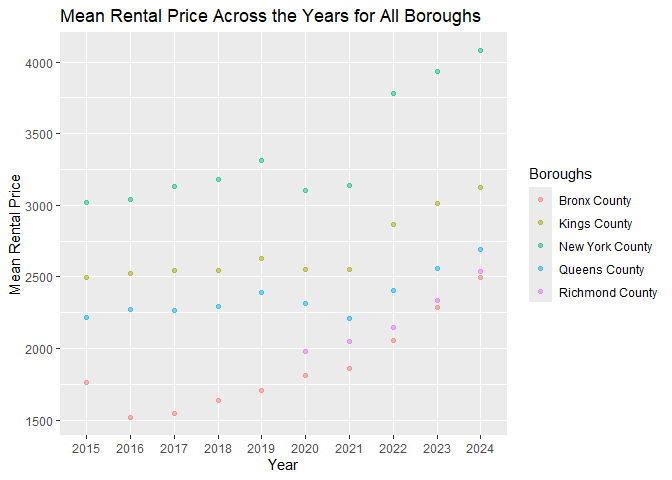
\includegraphics[keepaspectratio]{p8105_hw3_ry2539_files/figure-latex/mean_price_every_borough-1.pdf}}

In each of the boroughs, it seems like the mean rental price increases
from 2015 to 2024. For New York, Kings, and Queens County from 2019 to
2021, there seems to be a time when the rental price stayed relatively
unchanged or even decreased. This would make sense, as 2020 was the
start of the pandemic and therefore the demand for properties would have
decreased, decreasing the mean rental price for that year.

Comparing the trends across all boroughs, it seems that the mean rental
price for New York County a.k.a. Brooklyn is the highest. This would be
due to the demand for residential buildings there being much higher than
all other boroughs, especially in downtown Manhattan. Meanwhile, there
is a sharp increase in the mean rental price in Bronx county from 2017
to 2024. However, the mean rental price for Bronx County was still lower
than all other counties for every year.

This can be explained by examining how Bronx County has much more
available units for rent compared to New York county. Thus, this would
decrease the mean rental price for Bronx county compared to other
boroughs. It is also notable to see that while the mean rental price
dipped from 2019 to 2021 for New York, Queens, and King county, the mean
rental price kept increasing for Bronx and Richmond counties. However,
it is important to note that there is a lack of data for Richmond county
before 2020, thus lacking some comparability.

\begin{Shaded}
\begin{Highlighting}[]
\NormalTok{Zip\_Code\_Rent\_Year\_df }\OtherTok{=}\NormalTok{ Year\_pivot\_longer\_df }\SpecialCharTok{|\textgreater{}} \FunctionTok{mutate}\NormalTok{(}\AttributeTok{Year =} \FunctionTok{strtoi}\NormalTok{(Year))}

\CommentTok{\#Get rental price for every zip code that is observed\#}
  
\NormalTok{Zip\_Code\_Rent\_df }\OtherTok{=}\NormalTok{ Zip\_Code\_Rent\_Year\_df }\SpecialCharTok{|\textgreater{}} \FunctionTok{group\_by}\NormalTok{(Year, ZipCode, CountyName, Month) }\SpecialCharTok{|\textgreater{}} \FunctionTok{summarize}\NormalTok{(}\AttributeTok{rental\_price =} \StringTok{\textasciigrave{}}\AttributeTok{Rental Price}\StringTok{\textasciigrave{}}\NormalTok{, }\AttributeTok{na.rm =} \ConstantTok{TRUE}\NormalTok{)}
\end{Highlighting}
\end{Shaded}

\begin{verbatim}
## `summarise()` has grouped output by 'Year', 'ZipCode', 'CountyName'. You can
## override using the `.groups` argument.
\end{verbatim}

\begin{Shaded}
\begin{Highlighting}[]
\NormalTok{Zip\_Code\_Rent\_df }\OtherTok{=}\NormalTok{ Zip\_Code\_Rent\_df }\SpecialCharTok{\%\textgreater{}\%} \FunctionTok{mutate}\NormalTok{(}\AttributeTok{Date =} \FunctionTok{paste}\NormalTok{(}\FunctionTok{as.character}\NormalTok{(Year), }\FunctionTok{as.character}\NormalTok{(Month), }\AttributeTok{sep =} \StringTok{"{-}"}\NormalTok{))}

\CommentTok{\#separate data based on county name and plot it\#}

\NormalTok{every\_rent\_zip\_code }\OtherTok{=} \FunctionTok{ggplot}\NormalTok{(Zip\_Code\_Rent\_df, }\FunctionTok{aes}\NormalTok{(}\AttributeTok{x =}\NormalTok{ Date, }\AttributeTok{y =}\NormalTok{ rental\_price)) }\SpecialCharTok{+} \FunctionTok{geom\_point}\NormalTok{(}\FunctionTok{aes}\NormalTok{(}\AttributeTok{color =}\NormalTok{ ZipCode)) }\SpecialCharTok{+} \FunctionTok{facet\_wrap}\NormalTok{(}\SpecialCharTok{\textasciitilde{}}\NormalTok{CountyName) }\SpecialCharTok{+} \FunctionTok{labs}\NormalTok{(}\AttributeTok{title =} \StringTok{"Rental Price Within every Zip Code for All Available Years"}\NormalTok{, }\AttributeTok{x =} \StringTok{"Date"}\NormalTok{, }\AttributeTok{y =} \StringTok{"Rental Price"}\NormalTok{, }\AttributeTok{color =} \StringTok{"Zip Codes"}\NormalTok{)}

\NormalTok{every\_rent\_zip\_code}
\end{Highlighting}
\end{Shaded}

\begin{verbatim}
## Warning: Removed 26903 rows containing missing values or values outside the scale range
## (`geom_point()`).
\end{verbatim}

\pandocbounded{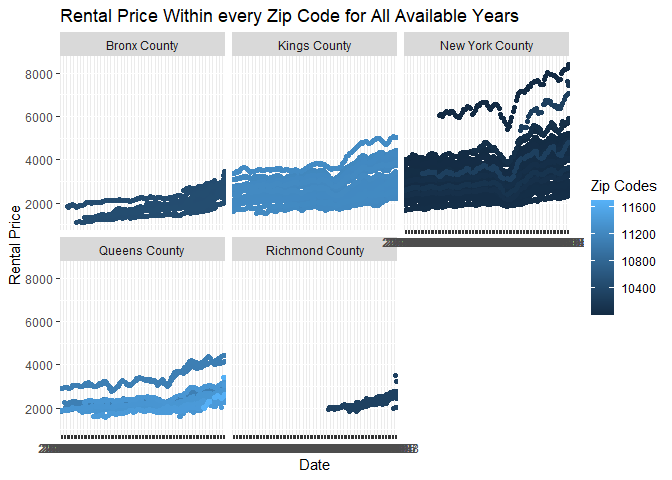
\includegraphics[keepaspectratio]{p8105_hw3_ry2539_files/figure-latex/rental_price_over_all_available_years-1.pdf}}

\begin{Shaded}
\begin{Highlighting}[]
\CommentTok{\#separate data based on zip code and export it to plot\#}

\NormalTok{p }\OtherTok{=} \FunctionTok{ggplot}\NormalTok{(Zip\_Code\_Rent\_df, }\FunctionTok{aes}\NormalTok{(}\AttributeTok{x =}\NormalTok{ Date, }\AttributeTok{y =}\NormalTok{ rental\_price)) }\SpecialCharTok{+} \FunctionTok{geom\_point}\NormalTok{(}\FunctionTok{aes}\NormalTok{(}\AttributeTok{color =}\NormalTok{ CountyName), }\AttributeTok{alpha =} \FloatTok{0.5}\NormalTok{) }\SpecialCharTok{+} \FunctionTok{facet\_wrap}\NormalTok{(}\SpecialCharTok{\textasciitilde{}}\NormalTok{ZipCode) }\SpecialCharTok{+} \FunctionTok{labs}\NormalTok{(}\AttributeTok{title =} \StringTok{"Rental Price Within every Zip Code for All Available Years"}\NormalTok{, }\AttributeTok{x =} \StringTok{"Date"}\NormalTok{, }\AttributeTok{y =} \StringTok{"Rental Price"}\NormalTok{, }\AttributeTok{color =} \StringTok{"Corresponding Borough"}\NormalTok{)}

\FunctionTok{ggsave}\NormalTok{(}\StringTok{"Results/zip\_codes\_borough.png"}\NormalTok{, }\AttributeTok{plot =}\NormalTok{ p, }\AttributeTok{width =} \DecValTok{30}\NormalTok{, }\AttributeTok{height =} \DecValTok{20}\NormalTok{, }\AttributeTok{limitsize =} \ConstantTok{FALSE}\NormalTok{)}
\end{Highlighting}
\end{Shaded}

\begin{verbatim}
## Warning: Removed 26903 rows containing missing values or values outside the scale range
## (`geom_point()`).
\end{verbatim}

After filtering out the zip codes and properties that were missing
values for rental prices, we observe the same trend of all properties
across boroughs increasing. The lack of data for earlier dates in
Richmond County could be attributed to how Staten Island may have had
properties that lacked units for rent. It is also notable that with
properties in New York County, there was a sharp decrease in the rental
price among many zip codes from the year 2019 to 2020. Again, this could
be attributed to the COVID-19 pandemic.

\begin{Shaded}
\begin{Highlighting}[]
\NormalTok{Twenty\_Twenty\_Three\_Zip\_Code\_rent\_df }\OtherTok{=}\NormalTok{ Zip\_Code\_Rent\_Year\_df }\SpecialCharTok{|\textgreater{}} \FunctionTok{filter}\NormalTok{(Year }\SpecialCharTok{==} \DecValTok{2023}\NormalTok{) }\SpecialCharTok{|\textgreater{}} \FunctionTok{group\_by}\NormalTok{(ZipCode, CountyName) }\SpecialCharTok{|\textgreater{}}  \FunctionTok{summarize}\NormalTok{(}\AttributeTok{mean\_rental\_price =} \FunctionTok{mean}\NormalTok{(}\StringTok{\textasciigrave{}}\AttributeTok{Rental Price}\StringTok{\textasciigrave{}}\NormalTok{)) }\SpecialCharTok{|\textgreater{}} \FunctionTok{drop\_na}\NormalTok{(mean\_rental\_price)}
\end{Highlighting}
\end{Shaded}

\begin{verbatim}
## `summarise()` has grouped output by 'ZipCode'. You can override using the
## `.groups` argument.
\end{verbatim}

\begin{Shaded}
\begin{Highlighting}[]
\CommentTok{\#make the plot that displays distribution of mean rental price over 2023 for zip codes\#}

\FunctionTok{ggplot}\NormalTok{(Twenty\_Twenty\_Three\_Zip\_Code\_rent\_df, }\FunctionTok{aes}\NormalTok{(}\AttributeTok{x =}\NormalTok{ ZipCode, }\AttributeTok{y =}\NormalTok{ mean\_rental\_price)) }\SpecialCharTok{+} \FunctionTok{geom\_point}\NormalTok{(}\FunctionTok{aes}\NormalTok{(}\AttributeTok{color =}\NormalTok{ CountyName), }\AttributeTok{alpha =} \DecValTok{1}\NormalTok{) }\SpecialCharTok{+} \FunctionTok{labs}\NormalTok{(}\AttributeTok{title =} \StringTok{"Mean Rental Price in 2023 and Zip Code"}\NormalTok{, }\AttributeTok{x =} \StringTok{"Zip Code"}\NormalTok{, }\AttributeTok{y =} \StringTok{"Mean Rental Price"}\NormalTok{, }\AttributeTok{color =} \StringTok{"Counties"}\NormalTok{)}
\end{Highlighting}
\end{Shaded}

\pandocbounded{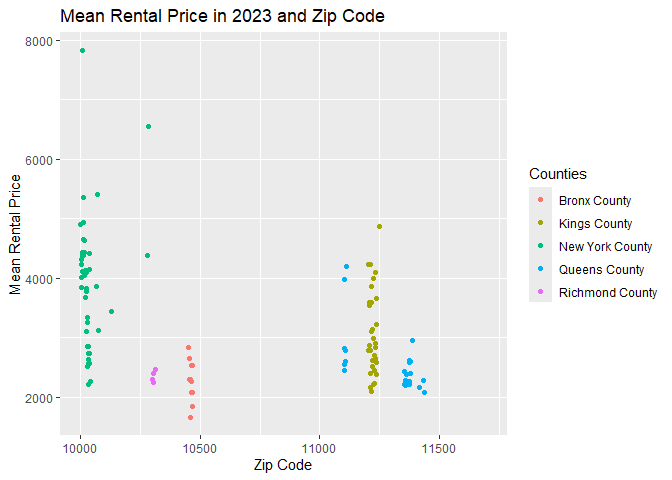
\includegraphics[keepaspectratio]{p8105_hw3_ry2539_files/figure-latex/plot_for_2023_rental_price-1.pdf}}

For the zip codes in New York County in 2023, the mean rental price has
a much larger dispersion compared to other boroughs. Specifically, it
has a couple of data points that have a mean rental price larger than
6,000 dollars per month. Overall, it seems like New York County has a
higher mean rental price in 2023 compared to other boroughs.

The second highest mean rental price belongs to Kings County, which
lines up with the trend observed for other years. It also lines up with
the mean rental price across all years for the boroughs.

Finally, the mean rental price over 2023 for Bronx County, Richmond
County, and Queens County is overall similar. It is notable that even in
2023, Richmond County has significantly less observations compared to
all other boroughs.

\begin{Shaded}
\begin{Highlighting}[]
\NormalTok{mean\_rent\_zip\_code\_2023\_plot }\OtherTok{=} \FunctionTok{ggplot}\NormalTok{(Twenty\_Twenty\_Three\_Zip\_Code\_rent\_df, }\FunctionTok{aes}\NormalTok{(}\AttributeTok{x =}\NormalTok{ ZipCode, }\AttributeTok{y =}\NormalTok{ mean\_rental\_price)) }\SpecialCharTok{+} \FunctionTok{geom\_point}\NormalTok{(}\FunctionTok{aes}\NormalTok{(}\AttributeTok{color =}\NormalTok{ CountyName))}

\NormalTok{combined\_plot }\OtherTok{=}\NormalTok{ every\_rent\_zip\_code}\SpecialCharTok{/}\NormalTok{mean\_rent\_zip\_code\_2023\_plot}

\FunctionTok{ggsave}\NormalTok{(}\StringTok{"Results/nyc\_combined\_rental\_trend.png"}\NormalTok{, }\AttributeTok{plot =}\NormalTok{ combined\_plot, }\AttributeTok{width =} \DecValTok{30}\NormalTok{, }\AttributeTok{height =} \DecValTok{20}\NormalTok{, }\AttributeTok{limitsize =} \ConstantTok{FALSE}\NormalTok{)}
\end{Highlighting}
\end{Shaded}

\begin{verbatim}
## Warning: Removed 26903 rows containing missing values or values outside the scale range
## (`geom_point()`).
\end{verbatim}

\section{Question 3}\label{question-3}

\begin{Shaded}
\begin{Highlighting}[]
\CommentTok{\#read our datasets\#}

\NormalTok{nhane\_covar\_df }\OtherTok{=} \FunctionTok{read\_csv}\NormalTok{(}\StringTok{"./Problem\_3\_Datasets/nhanes\_covar.csv"}\NormalTok{)}
\end{Highlighting}
\end{Shaded}

\begin{verbatim}
## New names:
## Rows: 254 Columns: 5
## -- Column specification
## -------------------------------------------------------- Delimiter: "," chr
## (5): ...1, 1 = male, ...3, ...4, 1 = Less than high school
## i Use `spec()` to retrieve the full column specification for this data. i
## Specify the column types or set `show_col_types = FALSE` to quiet this message.
## * `` -> `...1`
## * `` -> `...3`
## * `` -> `...4`
\end{verbatim}

\begin{Shaded}
\begin{Highlighting}[]
\NormalTok{nhane\_accel\_df }\OtherTok{=} \FunctionTok{read\_csv}\NormalTok{(}\StringTok{"./Problem\_3\_Datasets/nhanes\_accel.csv"}\NormalTok{)}
\end{Highlighting}
\end{Shaded}

\begin{verbatim}
## Rows: 250 Columns: 1441
## -- Column specification --------------------------------------------------------
## Delimiter: ","
## dbl (1441): SEQN, min1, min2, min3, min4, min5, min6, min7, min8, min9, min1...
## 
## i Use `spec()` to retrieve the full column specification for this data.
## i Specify the column types or set `show_col_types = FALSE` to quiet this message.
\end{verbatim}

\begin{Shaded}
\begin{Highlighting}[]
\CommentTok{\#clean, tidy, and merge our datasets\#}

\NormalTok{nhane\_covar\_clean\_variable\_df }\OtherTok{=}\NormalTok{ nhane\_covar\_df }\SpecialCharTok{|\textgreater{}} \FunctionTok{mutate}\NormalTok{(}\AttributeTok{SEQN =} \StringTok{\textasciigrave{}}\AttributeTok{...1}\StringTok{\textasciigrave{}}\NormalTok{, }\AttributeTok{sex =} \StringTok{\textasciigrave{}}\AttributeTok{1 = male}\StringTok{\textasciigrave{}}\NormalTok{,}
                                                      \AttributeTok{age =} \StringTok{\textasciigrave{}}\AttributeTok{...3}\StringTok{\textasciigrave{}}\NormalTok{, }\AttributeTok{BMI =} \StringTok{\textasciigrave{}}\AttributeTok{...4}\StringTok{\textasciigrave{}}\NormalTok{, }
                                                      \AttributeTok{education =} \StringTok{\textasciigrave{}}\AttributeTok{1 = Less than high school}\StringTok{\textasciigrave{}}\NormalTok{) }\SpecialCharTok{|\textgreater{}}
  \FunctionTok{select}\NormalTok{(}\SpecialCharTok{{-}}\StringTok{\textasciigrave{}}\AttributeTok{...1}\StringTok{\textasciigrave{}}\NormalTok{, }\SpecialCharTok{{-}}\StringTok{\textasciigrave{}}\AttributeTok{1 = male}\StringTok{\textasciigrave{}}\NormalTok{, }\SpecialCharTok{{-}}\StringTok{\textasciigrave{}}\AttributeTok{...3}\StringTok{\textasciigrave{}}\NormalTok{, }\SpecialCharTok{{-}}\StringTok{\textasciigrave{}}\AttributeTok{...4}\StringTok{\textasciigrave{}}\NormalTok{, }\SpecialCharTok{{-}}\StringTok{\textasciigrave{}}\AttributeTok{1 = Less than high school}\StringTok{\textasciigrave{}}\NormalTok{) }\SpecialCharTok{|\textgreater{}} \FunctionTok{drop\_na}\NormalTok{(SEQN, sex, age, BMI, education) }\SpecialCharTok{|\textgreater{}} \FunctionTok{filter}\NormalTok{(age }\SpecialCharTok{\textgreater{}=} \DecValTok{21}\NormalTok{) }\SpecialCharTok{|\textgreater{}} \FunctionTok{filter}\NormalTok{(SEQN }\SpecialCharTok{!=} \StringTok{"SEQN"}\NormalTok{) }\SpecialCharTok{|\textgreater{}} \FunctionTok{mutate}\NormalTok{(}
    \AttributeTok{sex =} \FunctionTok{case\_when}\NormalTok{(}
\NormalTok{      sex }\SpecialCharTok{==} \DecValTok{1} \SpecialCharTok{\textasciitilde{}} \StringTok{"male"}\NormalTok{,}
\NormalTok{      sex }\SpecialCharTok{==} \DecValTok{2} \SpecialCharTok{\textasciitilde{}} \StringTok{"female"}
\NormalTok{    ),}
    \AttributeTok{education =} \FunctionTok{case\_when}\NormalTok{(}
\NormalTok{      education }\SpecialCharTok{==} \DecValTok{1} \SpecialCharTok{\textasciitilde{}} \StringTok{"Less than high school"}\NormalTok{,}
\NormalTok{      education }\SpecialCharTok{==} \DecValTok{2} \SpecialCharTok{\textasciitilde{}} \StringTok{"High school equivalent"}\NormalTok{,}
\NormalTok{      education }\SpecialCharTok{==} \DecValTok{3} \SpecialCharTok{\textasciitilde{}} \StringTok{"More than high school"}
\NormalTok{    ),}
    \AttributeTok{SEQN =} \FunctionTok{as.numeric}\NormalTok{(SEQN), }\AttributeTok{age =} \FunctionTok{as.numeric}\NormalTok{(age), }\AttributeTok{BMI =} \FunctionTok{as.numeric}\NormalTok{(BMI)}
\NormalTok{  )}

\NormalTok{full\_nhane\_joint\_data\_df }\OtherTok{=} \FunctionTok{left\_join}\NormalTok{(nhane\_covar\_clean\_variable\_df, nhane\_accel\_df)}
\end{Highlighting}
\end{Shaded}

\begin{verbatim}
## Joining with `by = join_by(SEQN)`
\end{verbatim}

\begin{Shaded}
\begin{Highlighting}[]
\CommentTok{\#create table based on education and sex\#}

\NormalTok{table\_sex\_education\_distribution }\OtherTok{=}\NormalTok{ full\_nhane\_joint\_data\_df }\SpecialCharTok{|\textgreater{}} \FunctionTok{group\_by}\NormalTok{(sex, education) }\SpecialCharTok{|\textgreater{}}
  \FunctionTok{summarise}\NormalTok{(}\AttributeTok{n =} \FunctionTok{n}\NormalTok{()) }\SpecialCharTok{|\textgreater{}} \FunctionTok{pivot\_wider}\NormalTok{(}\AttributeTok{names\_from =}\NormalTok{ sex, }\AttributeTok{values\_from =}\NormalTok{ n)}
\end{Highlighting}
\end{Shaded}

\begin{verbatim}
## `summarise()` has grouped output by 'sex'. You can override using the `.groups`
## argument.
\end{verbatim}

\begin{Shaded}
\begin{Highlighting}[]
\NormalTok{table\_sex\_education\_distribution}
\end{Highlighting}
\end{Shaded}

\begin{verbatim}
## # A tibble: 3 x 3
##   education              female  male
##   <chr>                   <int> <int>
## 1 High school equivalent     23    35
## 2 Less than high school      28    27
## 3 More than high school      59    56
\end{verbatim}

\begin{Shaded}
\begin{Highlighting}[]
\CommentTok{\#Create distribution of counts of people for all ages\#}

\FunctionTok{ggplot}\NormalTok{(full\_nhane\_joint\_data\_df, }\FunctionTok{aes}\NormalTok{(}\AttributeTok{x =}\NormalTok{ age, }\AttributeTok{fill =}\NormalTok{ sex)) }\SpecialCharTok{+} \FunctionTok{geom\_histogram}\NormalTok{(}\AttributeTok{binwidth =} \DecValTok{4}\NormalTok{, }\AttributeTok{alpha =} \FloatTok{0.5}\NormalTok{) }\SpecialCharTok{+}
  \FunctionTok{facet\_grid}\NormalTok{(education}\SpecialCharTok{\textasciitilde{}}\NormalTok{sex) }\SpecialCharTok{+} \FunctionTok{labs}\NormalTok{(}\AttributeTok{title =} \StringTok{"Distribution of Ages Across Sexes and Education"}\NormalTok{, }\AttributeTok{x =} \StringTok{"Age"}\NormalTok{, }\AttributeTok{y =} \StringTok{"Count of People"}\NormalTok{, }\AttributeTok{color =} \StringTok{"Sex"}\NormalTok{)}
\end{Highlighting}
\end{Shaded}

\pandocbounded{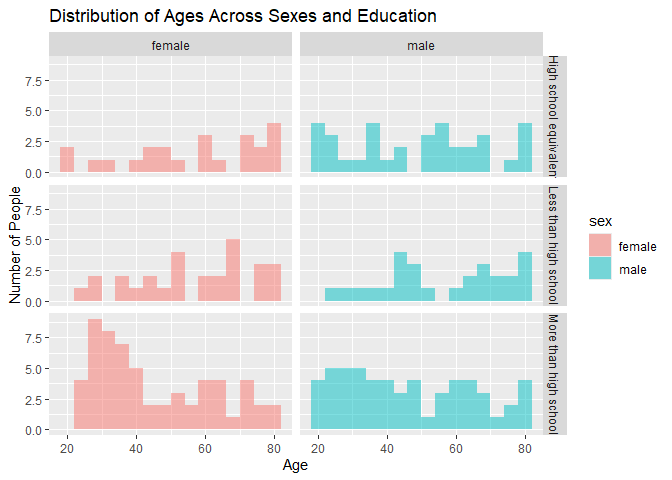
\includegraphics[keepaspectratio]{p8105_hw3_ry2539_files/figure-latex/visualisation_over_ages-1.pdf}}

For the participants with more than high school education, the
distribution of ages is skewed right for female participants compared to
male participants. This could be because how higher education was
historically dominated by male students and only relatively recently is
education being implemented more broadly across all sexes.

Meanwhile, the distribution of ages for less than high school education
is relatively concentrated around ages 45, 70,and 80 for male
participants, while the distribution for female participants in the same
education level is more uniform. The distribution for male participants
can be explained by how older participants may have come from a time
when people had less resources to study and attend higher education.
Overall, the total number of participants with this education level is
similar for both sexes.

Finally, the distribution of ages for an education of high school
equivalent is relatively uniform for both sexes. However, from the
table, we see that the total number of male participants are much higher
than female participants in this education level.

\begin{Shaded}
\begin{Highlighting}[]
\CommentTok{\#plot the total MIMS over all ages for sex and education levels\#}

\NormalTok{total\_MIMS\_df }\OtherTok{=}\NormalTok{ full\_nhane\_joint\_data\_df }\SpecialCharTok{|\textgreater{}} \FunctionTok{pivot\_longer}\NormalTok{(}\AttributeTok{cols =} \FunctionTok{starts\_with}\NormalTok{(}\StringTok{"min"}\NormalTok{), }
                                                        \AttributeTok{names\_to =} \StringTok{"MIMS"}\NormalTok{, }\AttributeTok{values\_to =} \StringTok{"MIMS amount"}\NormalTok{) }\SpecialCharTok{|\textgreater{}}
  \FunctionTok{group\_by}\NormalTok{(SEQN, sex, age, education) }\SpecialCharTok{|\textgreater{}} \FunctionTok{summarise}\NormalTok{(}\AttributeTok{Total\_MIMS =} \FunctionTok{sum}\NormalTok{(}\StringTok{\textasciigrave{}}\AttributeTok{MIMS amount}\StringTok{\textasciigrave{}}\NormalTok{))}
\end{Highlighting}
\end{Shaded}

\begin{verbatim}
## `summarise()` has grouped output by 'SEQN', 'sex', 'age'. You can override
## using the `.groups` argument.
\end{verbatim}

\begin{Shaded}
\begin{Highlighting}[]
\FunctionTok{ggplot}\NormalTok{(total\_MIMS\_df, }\FunctionTok{aes}\NormalTok{(}\AttributeTok{x =}\NormalTok{ age, }\AttributeTok{y =}\NormalTok{ Total\_MIMS, }\AttributeTok{color =}\NormalTok{ sex)) }\SpecialCharTok{+} \FunctionTok{geom\_point}\NormalTok{(}\AttributeTok{alpha =} \FloatTok{0.5}\NormalTok{) }\SpecialCharTok{+}
  \FunctionTok{geom\_smooth}\NormalTok{(}\AttributeTok{se =} \ConstantTok{FALSE}\NormalTok{) }\SpecialCharTok{+} \FunctionTok{facet\_grid}\NormalTok{(education}\SpecialCharTok{\textasciitilde{}}\NormalTok{sex)}\SpecialCharTok{+} \FunctionTok{labs}\NormalTok{(}\AttributeTok{title =} \StringTok{"Total MIMS Varied for All Ages"}\NormalTok{, }\AttributeTok{x =} \StringTok{"Age"}\NormalTok{, }\AttributeTok{y =} \StringTok{"Total MIMS"}\NormalTok{, }\AttributeTok{color =} \StringTok{"Sex"}\NormalTok{)}
\end{Highlighting}
\end{Shaded}

\begin{verbatim}
## `geom_smooth()` using method = 'loess' and formula = 'y ~ x'
\end{verbatim}

\pandocbounded{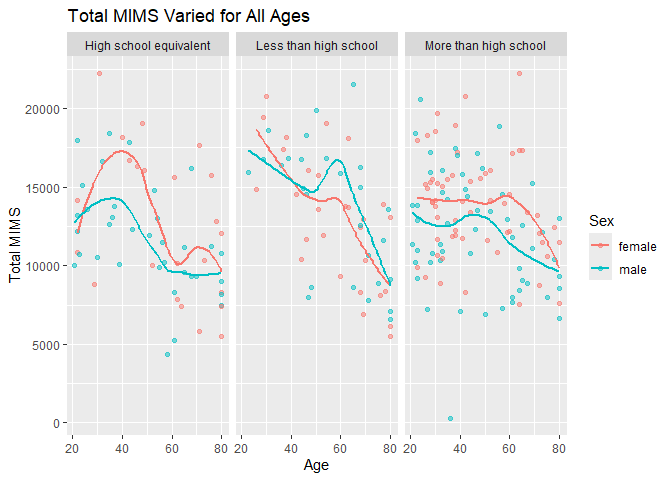
\includegraphics[keepaspectratio]{p8105_hw3_ry2539_files/figure-latex/total_MIMS_over_ages-1.pdf}}

For education levels, the total MIMS has an overall negative correlation
with age. For less than high school education, the total MIMS for all
ages is rather consistent between the sexes. However, for high school
equivalent education, there is an actual increase in total MIMS from
ages 20 to 40 for both male and female participants. The total MIMS for
female participants around age 40 is also significantly higher than male
participants. Finally, for more than high school education, the total
MIMS for female participants is higher than male participants by a bit
for all ages.

\begin{Shaded}
\begin{Highlighting}[]
\CommentTok{\#create a new dataset to transform each minute to their corresponding hour\#}

\NormalTok{time\_minute\_average\_df }\OtherTok{=}\NormalTok{ full\_nhane\_joint\_data\_df }\SpecialCharTok{|\textgreater{}} \FunctionTok{pivot\_longer}\NormalTok{(}\AttributeTok{cols =} \FunctionTok{starts\_with}\NormalTok{(}\StringTok{"min"}\NormalTok{), }
                                                        \AttributeTok{names\_to =} \StringTok{"MIMS"}\NormalTok{, }\AttributeTok{values\_to =} \StringTok{"MIMS amount"}\NormalTok{) }\SpecialCharTok{|\textgreater{}}
  \FunctionTok{mutate}\NormalTok{(}\AttributeTok{minute =} \FunctionTok{as.numeric}\NormalTok{(}\FunctionTok{str\_extract}\NormalTok{(MIMS, }\StringTok{"}\SpecialCharTok{\textbackslash{}\textbackslash{}}\StringTok{d+"}\NormalTok{)), }\AttributeTok{hour =}\NormalTok{ minute }\SpecialCharTok{\%/\%} \DecValTok{60}\NormalTok{) }\SpecialCharTok{|\textgreater{}} \FunctionTok{group\_by}\NormalTok{(hour, sex, education) }\SpecialCharTok{|\textgreater{}} \FunctionTok{summarise}\NormalTok{(}\AttributeTok{Mean\_MIMS =} \FunctionTok{mean}\NormalTok{(}\StringTok{\textasciigrave{}}\AttributeTok{MIMS amount}\StringTok{\textasciigrave{}}\NormalTok{))}
\end{Highlighting}
\end{Shaded}

\begin{verbatim}
## `summarise()` has grouped output by 'hour', 'sex'. You can override using the
## `.groups` argument.
\end{verbatim}

\begin{Shaded}
\begin{Highlighting}[]
\CommentTok{\#Plot out the average MIMS vs the hour of the day for all sexes and education levels\#}

\FunctionTok{ggplot}\NormalTok{(time\_minute\_average\_df, }\FunctionTok{aes}\NormalTok{(}\AttributeTok{x =}\NormalTok{ hour, }\AttributeTok{y =}\NormalTok{ Mean\_MIMS, }\AttributeTok{color =}\NormalTok{ sex)) }\SpecialCharTok{+} \FunctionTok{geom\_point}\NormalTok{(}\AttributeTok{alpha =} \FloatTok{0.5}\NormalTok{) }\SpecialCharTok{+}
  \FunctionTok{geom\_smooth}\NormalTok{(}\AttributeTok{se =} \ConstantTok{FALSE}\NormalTok{) }\SpecialCharTok{+} \FunctionTok{facet\_wrap}\NormalTok{(}\SpecialCharTok{\textasciitilde{}}\NormalTok{education)}\SpecialCharTok{+} \FunctionTok{labs}\NormalTok{(}\AttributeTok{title =} \StringTok{"Average MIMS for Every Hour Depending on Education Level"}\NormalTok{, }\AttributeTok{x =} \StringTok{"Hour of the Day"}\NormalTok{, }\AttributeTok{y =} \StringTok{"Average MIMS"}\NormalTok{, }\AttributeTok{color =} \StringTok{"Sex"}\NormalTok{)}
\end{Highlighting}
\end{Shaded}

\begin{verbatim}
## `geom_smooth()` using method = 'loess' and formula = 'y ~ x'
\end{verbatim}

\pandocbounded{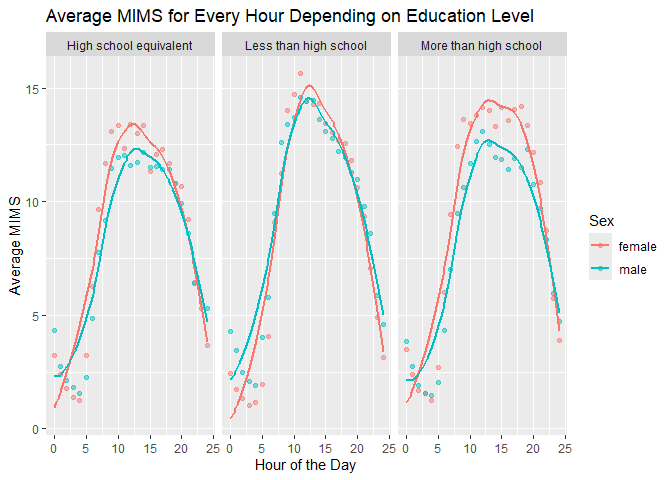
\includegraphics[keepaspectratio]{p8105_hw3_ry2539_files/figure-latex/average_MIMS_over_hour_of_day-1.pdf}}

Overall, it seems that the mean MIMS increases from midnight to around
noon of the day, and then decreases from noon to midnight. The more
notable differences can be observed between the sexes. For less than
high school education, the mean MIMS is similar for both female and male
participants. However, for high school equivalent and higher education,
the mean MIMS is higher for female participants over male participants.

For higher than high school education, the mean MIMS for female
participants is much higher than male participants around the hours of
10 to 20. The same trend can be observed for high school equivalent
education, although the discrepancy between the sexes is much smaller.
For other hours, the mean MIMS of female participants are only higher
than male participants by a percentage at most. Otherwise, the mean MIMS
difference is rather insignificant between the sexes.

\end{document}
